%%This is a very basic article template.
%%There is just one section and two subsections.
\documentclass[pdftex,11pt,a4paper]{article}

\usepackage{graphicx}
\usepackage{float}
\usepackage{indentfirst}
\usepackage{url}

\usepackage{amssymb, amsmath}

\usepackage[T1]{fontenc} % font encoding
\usepackage[utf8]{inputenc} % input encoding
\usepackage[english]{babel} % keyword translation and hyphenation
\usepackage{lmodern} % lmodern looks better than cm-super

\usepackage[none]{hyphenat}%%%%

\usepackage{color, colortbl}
\definecolor{Gray}{gray}{0.9}
\definecolor{LightCyan}{rgb}{0.88,1,1}

\usepackage[first=0,last=9]{lcg}
\newcommand{\ra}{\rand0.\arabic{rand}}

\usepackage[table]{xcolor}% http://ctan.org/pkg/xcolor
\begin{document}

\title{Analyzing Model to Model Transformation
	   Tools}
\date{April 23}
\author{Petter Barvik}

\maketitle

\abstract{}

\newpage
\section{Introduction}

\noindent Model Driven Engineering (MDE)\cite{France2007} thrives to raise the
level of abstraction in program specification and increase automation in program
development. The main idea for MDE is to use models at different levels of
abstraction when developing applications. This leads to a higher level
of abstraction in program and problem specification. This level of abstraction
is obtained either through extensive use of models to describe some design
patterns in a software application or through use of standardized models. The
first option is probably an element of MDE that is most common among software
engineers. That you implement some aspect of a system based on a model of a 
specific language. Unified Modelling Language is an example of a modelling
language often used to describe system design patterns in an application
domain. The second principle of Model Driven Engineering is to increase
automation in program development, and to obtain this we use something called
model transformations. \\
\indent A model transformation is when we change some source model from one
instance to another instance and end up with a target model. We can
distinguish these operations into either endogenous or exogenous model
transformations. In an endogenous model transformation we take one model
expressed in a language and produce a model expressed in the same language.
While in an exogenous model transformation we start with a model
expressed in one language and translate this into a model expressed in another
language. It is essential that these models are consistent. This is obtained
through the use of metamodels. A metamodel is a description of a model, where
it defines elements that are used in the model. Models in a system is consistent
if the source and target model corresponds to a metamodel. This way system
developers can safely presume that a model has changed accordingly to its
metamodel and therefore is consistent. A target model can produce two different
kind of output models. The first one is code generation, often referred to
Model to Text(M2T) transformation, and it takes one model and produces
implementation code. This is convenient if for example a software engineer
wants to produce source code from a given model. The latter is often referred
to Model to Model(M2M) transformations. M2M transformations take a model as
input and produces a model as output. In this article we try and go into depth
for some model to model transformation tools. These tools are
Henshin\cite{Henshin}, AGG\cite{AGG} and ATL\cite{ATL}. Henshin and AGG is
build around graph transformation.

% Er det ikke mer � se p� en eksempel model transformasjon og hvordan den kan
% utf�res i forskjellige verkt�y? Etterp� evalurer du verkt�yene med tanke p�
% styrker og svakheter. S� kan du forklare eksemplet etterp�.

Model-to-model transformation is a key aspect of model-driven development (MDD).
The MMT project provides a framework for model-to-model transformation
languages. Transformations are executed by transformation engines. There are
three transformation engines that are developed in the scope of this project:
ATL, QVTo, QVTd. MMT is a subproject of the top-level Eclipse Modeling Project.

\subsection{Problem specification}
\noindent In this article we look at a specific example of a model to model
transformation and evaluate how this example performs for different tools.
When we have applied this example to the different tools, we will try and
find both strengths and weaknesses for these tools. The task was to take a
certain instance of a model to model transformation, in this case translating
an activity diagram, written in the language UML, and transform it to a petri
net model. We initialize the metamodels to make sure that the models remain
consistent. These metamodels are represented in the Ecore
model\cite{Steinberg2009}. The Ecore model is used to represent models in EMF.
Ecore itself is an EMF model, and therefore has its own metamodel. You could say
that this makes Ecore a meta-metamodel, since the two metamodels below are
represented in Ecore.

\begin{figure}[H]
	\centering
	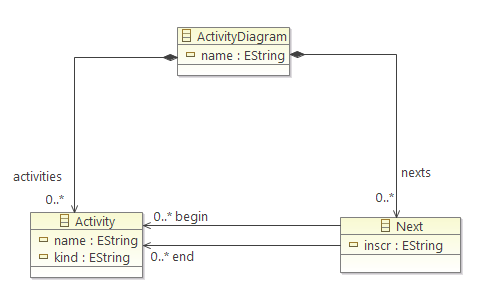
\includegraphics[scale=0.5]{figures/ActivityMetamodel.png}
	\caption{Metamodel of Activity Diagram.}
	\label{fig:ActivityMetamodel}
\end{figure}

The metamodel of an activity diagram has an arbitrary number of activities and
next elements. An activity element can have a name and a kind.
Example of activity types can be decision or simple. The next element can have
an inscription and has the property to either start or end activities. The
collection of activities and next elements have to have an activity diagram that
they belong to. Now we have defined the metamodel that the source model should
conform to. To keep consistency between the models we need to have a
metamodel for the target model.

\begin{figure}[H]
	\centering
	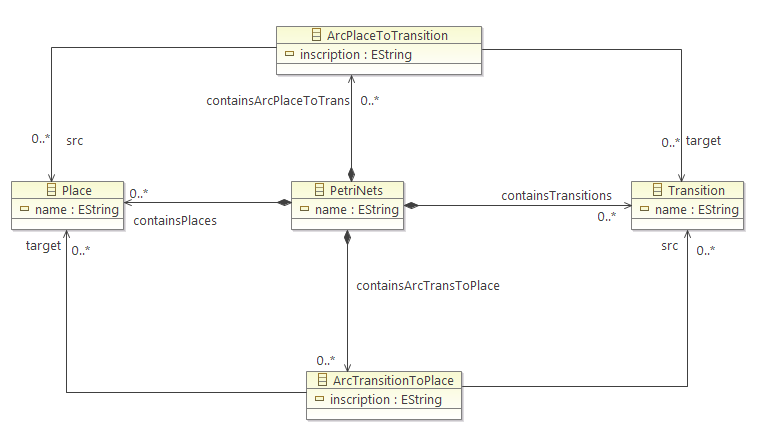
\includegraphics[scale=0.5]{figures/PetriNetsMetamodel.png}
	\caption{Metamodel of Petri nets.}
	\label{fig:PetriNetsMetamodel}
\end{figure}

The metamodel for a petri net consist of places and transitions. A petri net
instance must have a place connected to a transition or the other way around.
But a petri net can never have two of the same types connected with each other.
To solve this, the petri net metamodel has two nodes that specify if the
connection is between a place and a transition or a transition and a place.
\indent Now that we have defined the two corresponding metamodels, we can use
these two ecore models in both Henshin and ATL. These two transformation
languages provides support the Ecore meta-metamodel technology, defined by
Eclipse Modelling Framework. 

\section{Graph Transformation}
\noindent One approach to model transformations is by graph transformations,
also referred to as graph rewriting. And one approach to graph rewriting is an algebraic
approach, which is based upon category theory\cite{Barr1990}.

\begin{figure}[H]
	\centering
	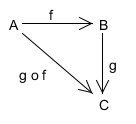
\includegraphics[scale=0.7]{figures/categoryTheory.png}
	\caption{Collection of objects A,B and C.}
	\label{fig:categoryTheory}
\end{figure}


In category theory there are a collection of objects and arrows. These arrows
are also called morphisms. In figure~\ref{fig:categoryTheory} we have a
collection of objects A, B and C and morphisms f, g and g $\circ$ f. And for the
purpose of this paper, the collection of objects are graphs and the arrows are
graph morphisms. This is also very typical when writing papers to explain the
concepts of graph transformations, where these objects are represented as graphs, and
arrows are represented as morphisms. Category theory can then be used to
formalize the concepts at a high level of abstraction.

\subsection{The Algebraic Approach}
\noindent This approach are based on the concepts of gluing of graphs, modelled
by pushouts of graphs and graph morphisms. These pushouts comes in different
categories, and we will look at two approaches to graph transformations, namely
the double-pushout (DPO) approach and the single pushout (SPO)
approach\cite{Loewe1997,Ehrig1997}.

\indent Historically, the first of the algebraic approaches to graph
transformations, the double-pushout, was first introduced at the Technical
University of Berlin in the early seventies by H. Ehrig, M. Pfender and H.J.
Schneider\cite{INSPEC:606170}. They tried to generalize Chromsky grammars from
strings to graphs. This allowed to define a graph rewriting step by the use of
two gluing constructions. And by applying a graph rewriting step for the
double-pushout approach is a pair of morphisms in the category of graphs where
the arrows represents total graph morphisms, \linebreak\mbox{L $\longleftarrow$
\ K $\longrightarrow$ R}. This is true for each application rule in a graph
transformation for the double-pushout approach. Where the graph K represents the
gluing part and the two morphisms \mbox{L $\longleftarrow$ \ K} and \mbox{K
$\longrightarrow$ R} use the algebraic construction, pushout to apply an
application rule for a rewriting step. Hence the name double pushout and the use
of two gluing conditions.


\subsection{Productions}
\noindent For a transformation language to be able to execute for graph
transformations a set of application rules needs to be defined. Through these
rules, a transformation interpreter can act accordingly. These rules are often
referred to as Productions. For graph transformations, there can be an arbitrary
number of rules. Its truly up to the users how they want to translate a
language and how many rules that is needed to acquire this. Each rule consists
of a left hand side (LHS) and a right hand side (RHS), also often referred to as
pattern graph and replacement graph. The pattern graph represents a subgraph of
the model that is going to be translated, namely the host graph.
% \indent These productions are handled 

\subsection{A Direct Derivation}
\noindent The basic idea for graph transformation for both the double-pushout
approach and the single pushout approach is to apply an application rule
\mbox{r: L $\longrightarrow$ R}. Where the rule represents a single rewriting
step for graph transformations and L represents the left hand side of the rule and R
represents the right hand side of the rule.

\begin{figure}[H]
	\centering
	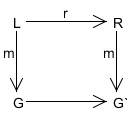
\includegraphics[scale=0.7]{figures/GraphTransformationGeneral.png}
	\caption{The basic idea for graph transformation by applying a rule r.}
	\label{fig:GraphTransformationGeneral}
\end{figure}

For a production rule r, \mbox{G$\xrightarrow{r,m}$G'} indicates a direct
derivation to a derived graph G'. If there is a match m of nodes and arrows for a
subgraph L in a host graph G, then this indicates a graph homomorphism, mapping
elements from the subgraph to the host graph in such a way that the graphical
structure in G is preserved.

\section{The Attributed Graph Grammar System}

\noindent AGG is a general development environment for algebraic graph
transformation systems. AGG is provided with a graphical editor for creating
and modifying graphs. The editor provides a graphical user-interface with
several visual editors for applying the principles of graph transformation. It
also has an interpreter and a set of validation tools.

\subsection{Graphical Editor}
\noindent The graphical editor of AGG has several functions to help the user to
define model transformations. In the top left corner of the graphical user-interface is
a tree based editor for defining rules and grammar. This tree based editor also
contains the type graphs and the host graphs. Where the host graph represents
some input model for a model transformation.

\indent Each application rule has two visual editors, representing the left and
the right hand side, or the pattern and the replacement graph. In the tree
collection of rules and grammars it is possible to give rules application
conditions. This is convenient if the user wants to have constrains for the
pattern or the replacement graph. 

\indent In the tree based visual editor it is also possible to define host
graphs and type graphs. Type graphs is described more in depths in the next
section, but roughly said, the type graph defines elements that can be used in
the host graph. Type graphs defines the abstract models for the host graph and
can be compared to Meta Object Facility (MOF)\cite{MOF}, that is a language for
defining abstract syntax of modeling languages. The users can now create instances
from these type graphs. These instances represents the host graphs and
corresponds to its concurrent type graph. 

\indent For the application rules, the user can extend the attributes with Java
expressions. This means that the users can use Java primitives such as strings,
integers or float numbers to form the pattern graph or the left hand side of the
rule. The user cannot bind attributes that is not initialised in the type graph. 

\subsection{Type Graph}

\noindent Before the host graphs can be created. a type graph has to be
initialised. These type graphs represents the abstract syntax for the host
graphs. For this case study we created a type graph enabling translation from
an activity diagram to petri nets. Unlike Henshin, the AGG graphs does not
allow for separately definitions of type graphs. Henshin allows the use of one
source and one target metamodel independent of each other. If we want to
prepare an AGG graph for a transformation, we create a single type graph with
references between elements of both source and target metamodel. This way, when
the application rules is executed, we can choose to keep both the source graph
and the references between these elements. The references and source graph can
be deleted through a cycle of transformation rules.

\begin{figure}[H]
	\centering
	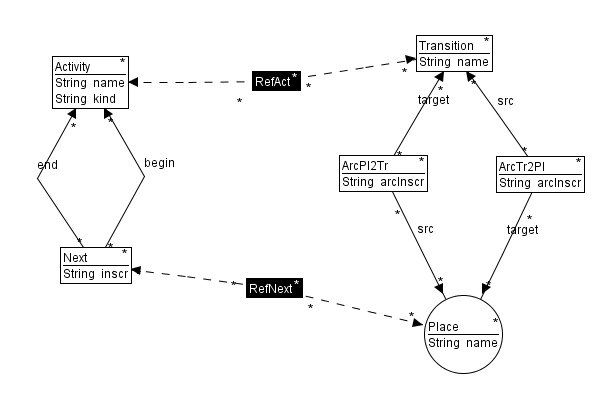
\includegraphics[scale=0.7]{figures/AggTypeGraph.png}
	\caption{Activity diagram to petri nets type graph in AGG.}
	\label{fig:AggTypeGraph}
\end{figure}

\indent For the type graph, the user must define nodes and arrows for each
element for both source and target model. These nodes and arrows can also have
attributes. Nodes represents elements from the two modelling languages and
arrows represents the associations between these elements. In the type graph we
want to distinguish between associations and references, and therefore we
represent references as a dashed edge. These dashed edges are not given any
attributes, and that is because we want these edges to represent what the
targeted element was translated from. From figure~\ref{fig:AggTypeGraph} we can
see that a RefAct node is defined and is connected between the activity
element and the transition element. The same initialisation is defined between
the place next element and the place element. The elements presented in the
type graph for AGG graphs is very similar to the metamodels represented for
Henshin transformations. For AGG type graphs there is a multiplier condition for
the edges. This means that there can be an arbitrary, or a zero to many number of
instances of these relations in the host graph.

\section{The Henshin Project}

\noindent The Henshin project\cite{Henshin} provides a model transformation
language for the Eclipse Modelling Framework \cite{Steinberg2009}. With support for both direct 
transformation of EMF single model instances, and translation from source
model to targeted model. The Henshin project is a transformation language with a
provided graphical syntax. With the help of this graphical editor, it provides
the user with an intuitive way of representing rules. 

\subsection{Graphical Editor}
\noindent Henshin model transformation language is a plugin for the Eclipse
Integrated Development Environment\cite{Eclipse}. The Henshin project provides
the users with a graphical editor to create and modify model to model
transformations. 

The users start out with using the Eclipse wizard to create an empty Henshin
document. The henshin document is based on the commonly known Extensible Markup
Language (XML)\cite{XML}. If applicable a Henshin diagram file can be created
based on the Henshin file. This gives the users an intuitive approach to
creating model transformation rules.

The Henshin transformation file is represented in a tree based editor in
Eclipse. In this tree based editor it is possible to include metamodels for both
the source and the target model. These metamodels are created based on the EMF
standard for creating models, that we talked about in the first chapter.
This approach differ from the AGG approach we saw in section 3, where we have
to create both target and source metamodel in one common type graph. In Henshin
the two metamodels are independent of one and another, therefore they are
included as two separate models in the Henshin file. 

\subsection{Defining transformation rules}

\noindent In Henshin, objects are referred to as nodes and links between objects
as edges. A collection of these nodes and edges form a graph. For each graph, a
rule has to be defined. These rules can have parameters for checking and model
verification. Each rule can be represented as a graph in the graphical
editor. 

\indent When creating these rules, there has to be a way of
distinguishing elements between the LHS and the RHS. This is done through the use of
a set of predefined tag words, or stereotypes. For handling transformations
either in the pattern graph or the replacement graph, we can use the three
predefined words <<preserve>>, <<create>> or <<delete>>. <<forbid>> and
<<require>> are used for defining Negative Application Conditions (NACs) and
Positive Application Conditions (PACs). These actions are supported for nodes,
edges and attributes. 

\section{ATL Transformation Language}

\noindent ATL\cite{ATL} (ATL Transformation Language) is a model transformation
language. It provides ways to produce a set of target models from a set of
source models. ATL is developed on top of the Eclipse platform and is one of
three transformation engines provided by the MMT project\cite{MMT}. MMT is a
sub project of the top level Eclipse Modeling Project\cite{EMP}. 

A metametamodel aims to introduce the semantics that are required to specify
metamodels. As a  model with its metamodel, a metamodel conforms to the
metametamodel. Note that a metametamodel is usually self-defined, which means
that it can be specified by means of its own semantics. In such a case, a
metametamodel conforms to itself.


Several metametamodel technologies are available. The ATL transformation engine
currently provides support for two of these existing technologies: the Meta
Object Facilities (MOF 1.4) defined by the OMG and the Ecore metametamodel
(Budinsky, F., Steinberg, D., Ellersick, R., Grose, T. Eclipse Modeling
Framework, Chapter 5 "Ecore Modeling Concepts". Addison Wesley Professional.
ISBN: 0131425420, 2004) defined by the Eclipse Modeling Framework (EMF). This
means that ATL is able to handle metamodels that have been specified according
to either the MOF or the Ecore semantics.

\subsection{Syntax based editor}

\noindent ATL 

Model-to-model transformation is a key aspect of model-driven development (MDD).
The MMT project provides a framework for model-to-model transformation
languages. Transformations are executed by transformation engines. There are
three transformation engines that are developed in the scope of this project:
ATL, QVTo, QVTd. MMT is a subproject of the top-level Eclipse Modeling Project.

syntax-based transfor-
mation language

\begin{figure}[H]
	\centering
	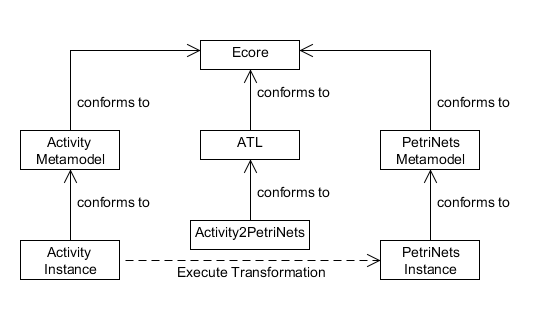
\includegraphics[scale=0.5]{figures/ATL.png}
	\caption{Model transformation process for Activity2PetriNets.}
	\label{fig:ATL}
\end{figure}

This schema provides an overview of the ATL transformation (Author2Person) that
enables to generate a Person model, conforming to the metamodel MMPerson, from
an Author model that conforms to the metamodel MMAuthor. The designed
transformation, which is expressed by means of the ATL language, conforms to
the ATL metamodel. In this example, the three metamodels (MMAuthor, MMPerson
and ATL) are expressed using the semantics of the Ecore metametamodel.




\section{Evaluation}
The tool also has support 
both endogenous and exogenous transformations.

\begin{table}[ht]
\centering
\begin{tabular}{| c | c | c | c | c |}
\hline
&Values & AGG & Henshin & ATL \\
\hline
Endogenous transformation& Yes / No & \cellcolor{green!25}Yes &
\cellcolor{green!25}Yes & \cellcolor{green!25}Yes \\

Exogenous transformation& Yes / No & \cellcolor{green!25}Yes &
\cellcolor{green!25}Yes & \cellcolor{green!25}Yes \\

Input Elements& 1 to n & 1\ldots n & 1\ldots n & 1\ldots n\\
Output Elements & 1 to n & 1\ldots n & 1\ldots n & 1\ldots n\\
Graphical syntax& Yes / No &\cellcolor{green!25}Yes &
\cellcolor{green!25}Yes &\cellcolor{red!25}No  \\
Creates target model isntances & Yes / No &\cellcolor{red!25}No &
\cellcolor{red!25}No &\cellcolor{green!25}Yes \\
Integrated with Java& Yes / No & \cellcolor{green!25}Yes &
\cellcolor{green!25}Yes & \cellcolor{green!25}Yes \\
Supports EMF& Yes / No & \cellcolor{red!25}No &
\cellcolor{green!25}Yes & \cellcolor{green!25}Yes \\
Seperate metamodels& Yes / No & \cellcolor{red!25}No &
\cellcolor{green!25}Yes & \cellcolor{green!25}Yes \\
\hline

\end{tabular}
\end{table}

\pagebreak
\bibliographystyle{ieeetr} 
\bibliography{master,websites}

\end{document}